\documentclass{article}
\usepackage[preprint]{neurips_2025}

\usepackage[utf8]{inputenc}
\usepackage[T1]{fontenc}
\usepackage{hyperref}
\usepackage{url}
\usepackage{booktabs}
\usepackage{amsfonts}
\usepackage{amsmath}
\usepackage{microtype}
\usepackage{xcolor}
\usepackage{graphicx}
\usepackage{subcaption}
\usepackage{multirow}
% \usepackage{tablefootnote}

\title{The Geometry of SFT Perturbations: Direction, Not Magnitude, Determines Degradation}

\author{
  Anonymous Authors
}

\begin{document}

\maketitle

\begin{abstract}
Supervised fine-tuning (SFT) with LoRA perturbs pre-trained weights by a low-rank update $\Delta W$. The conventional assumption is that degradation depends on the \emph{magnitude} of this perturbation: larger $\|\Delta W\|$ means more forgetting. Through an 84-experiment study fine-tuning Qwen2.5-3B-Instruct on math chain-of-thought data from four sources, we show this is only half the story. Within a data source, perturbation norm strongly predicts accuracy degradation ($R^2 = 0.94$ for NuminaMath, $0.86$ for NuminaMath-Hard, $0.80$ for OpenR1). But across sources, the same norm produces vastly different outcomes: NuminaMath at $\|\Delta W\| = 0.87$ yields 20\% ORZ accuracy, while OpenR1 at $\|\Delta W\| = 0.79$ yields 5.4\%---a 4$\times$ degradation gap at comparable perturbation magnitude. We explain this through \textbf{perturbation direction analysis}: pairwise cosine similarity between LoRA weight updates reveals that data sources occupy distinct directions in weight space (intra-source cosine ${\sim}0.88$, cross-source cosine ${\sim}0.50$), and these directions diverge as training volume increases (cosine drops from 0.75 at $N{=}100$ to 0.24 at $N{=}10{,}000$). We further decompose degradation into format disruption (transient, exhibiting phase-transition dynamics) and reasoning degradation (cumulative, monotonic), showing that OpenR1's direction causes catastrophic format collapse between $N{=}1{,}500$ and $N{=}2{,}000$. We validate these findings across two model scales (3B and 7B) and show that non-math SFT (code generation) produces near-orthogonal perturbation directions ($\cos{\sim}0.01$), confirming the framework extends beyond math-variant data sources.
\end{abstract}

%---------------------------------------------------------------------
\section{Introduction}
%---------------------------------------------------------------------

Supervised fine-tuning (SFT) with LoRA~\citep{hu2022lora} is the standard method for specializing instruction-tuned language models. A natural question is: how much degradation does SFT cause on the model's existing capabilities? The conventional answer focuses on \emph{magnitude}---larger weight perturbations should cause more forgetting.

We present evidence that this magnitude-centric view is fundamentally incomplete. Consider two SFT experiments with comparable perturbation norms:
\begin{itemize}
    \item \textbf{NuminaMath $N{=}10{,}000$}: $\|\Delta W\|_F = 0.87$, ORZ accuracy $= 20.0\%$
    \item \textbf{OpenR1 $N{=}2{,}000$}: $\|\Delta W\|_F = 0.79$, ORZ accuracy $= 5.4\%$
\end{itemize}
OpenR1 achieves a 3.7$\times$ worse outcome at a \emph{smaller} perturbation magnitude. This cannot be explained by norm alone---NuminaMath at $\|\Delta W\| = 0.60$ ($N{=}2{,}000$) maintains 23.3\% accuracy, while OpenR1 at the larger $\|\Delta W\| = 0.79$ collapses to 5.4\%.

We resolve this paradox by analyzing the \textbf{direction} of LoRA perturbations. Computing pairwise cosine similarity between weight update vectors across 84 checkpoints reveals three key findings:

\textbf{(F1) Data sources produce distinct perturbation directions.} Intra-source cosine similarity averages 0.88 (NuminaMath) and 0.72 (OpenR1), while cross-source similarity averages only 0.50.

\textbf{(F2) Perturbation directions diverge with training volume.} At $N{=}100$, NuminaMath and OpenR1 directions are moderately aligned (cosine $= 0.75$). By $N{=}10{,}000$, they are nearly orthogonal (cosine $= 0.24$).

\textbf{(F3) Direction determines degradation rate per unit norm.} Within each source, norm strongly predicts accuracy ($R^2 > 0.80$). But the \emph{slope} differs across sources: each unit of OpenR1 perturbation causes more damage than the equivalent NuminaMath perturbation.

\paragraph{Contributions.}
(1)~A geometric framework for SFT degradation where perturbation direction, not just magnitude, determines which capabilities degrade.
(2)~Empirical evidence from 84 experiments showing source-dependent directions, $N$-dependent divergence, and source-dependent degradation rates.
(3)~Decomposition of degradation into format disruption (transient) and reasoning degradation (cumulative), with format disruption contributing 73\% of peak loss.
(4)~Intervention experiments: truncating OpenR1 solutions and mixing data sources smoothly interpolates perturbation directions and outcomes.
(5)~Validation across two model scales (3B, 7B) and cross-domain SFT (code generation).

%---------------------------------------------------------------------
\section{Related Work}
%---------------------------------------------------------------------

\textbf{Catastrophic forgetting in continual learning.} The standard framing focuses on cross-task interference~\citep{kirkpatrick2017overcoming, luo2023empirical}. EWC and experience replay are common mitigations. We show that under LoRA SFT at this scale, cross-domain forgetting is largely mitigated---the binding constraint is direction-dependent intra-domain degradation.

\textbf{Weight perturbation theory.} Random perturbation studies~\citep{li2018measuring} establish that neural networks tolerate perturbations below a scale-dependent threshold. Our contribution is showing that for \emph{structured} perturbations (LoRA SFT), direction matters more than scale, with different data sources producing perturbations in distinct weight-space subspaces.

\textbf{LoRA and parameter-efficient fine-tuning.} \citet{hu2022lora} showed LoRA preserves most pre-trained capabilities through low-rank updates. \citet{biderman2024lora} studied LoRA for continual learning. We extend this by analyzing the geometric structure of LoRA perturbations across data sources, revealing source-dependent directional signatures.

\textbf{Data scaling and selection for SFT.} LIMA~\citep{zhou2023lima} and AlpaGasus~\citep{chen2023alpagasus} study how data quantity and quality affect SFT outcomes. We add a geometric perspective: not just \emph{how much} data, but \emph{which direction} the resulting perturbation points determines the outcome.

%---------------------------------------------------------------------
\section{Experimental Setup}
%---------------------------------------------------------------------

\subsection{Model and Training}

We fine-tune \textbf{Qwen2.5-3B-Instruct}~\citep{yang2024qwen} using LoRA applied to all attention projections (Q, K, V, O) across 36 transformer layers (144 LoRA modules). Standard configuration: rank $r{=}8$, learning rate $5{\times}10^{-5}$, 1 epoch, effective batch size 16, cosine schedule, bfloat16 precision. For scale generality, we additionally fine-tune \textbf{Qwen2.5-7B-Instruct}.

\subsection{Data Sources}

All training data consists of math chain-of-thought solutions with \texttt{\textbackslash boxed\{\}} answer formatting.

\begin{table}[h]
\centering
\caption{Training data sources. All contain math CoT solutions.}
\label{tab:sources}
\small
\begin{tabular}{@{}llrl@{}}
\toprule
Source & Description & Mean Length & Characteristic \\
\midrule
NuminaMath & Random sample from 860K CoT & 1,150 chars & Textbook-style, concise \\
NuminaMath-Hard & Competition problems & 2,081 chars & Detailed competition solutions \\
OpenR1 & DeepSeek R1 distillation traces & 16,469 chars & Extended reasoning, 14$\times$ longer \\
CodeAlpaca & 20K coding instructions & ${\sim}500$ chars & Code generation, non-math \\
\bottomrule
\end{tabular}
\end{table}

\subsection{Evaluation}

\begin{table}[h]
\centering
\caption{Evaluation benchmarks and baselines (Qwen2.5-3B-Instruct).}
\label{tab:benchmarks}
\small
\begin{tabular}{@{}llrr@{}}
\toprule
Benchmark & Domain & Size & Baseline \\
\midrule
ORZ Math & Competition math & 1,024 & 28.91\% \\
GSM8K & Grade-school math & 1,319 & 84.00\% \\
SciKnowEval & Chemistry MCQ & 1,893 & 34.34\% \\
ToolAlpaca & Tool-use & 192 & 89.22\% \\
\bottomrule
\end{tabular}
\end{table}

We evaluate in both \emph{strict} mode (\texttt{\textbackslash boxed\{\}} extraction only) and \emph{tolerant} mode (fallback to last number). The gap isolates format-dependent degradation.

\subsection{Experiment Design}

We conduct 84 experiments spanning: sample counts $N = 50$ to $10{,}000$; 4 math data sources plus CodeAlpaca; multiple LoRA configurations ($r \in \{4, 8, 16, 32\}$); 4 random seeds at key sample counts; truncation controls; data mixing at varying ratios; and 7B-scale replication.

%---------------------------------------------------------------------
\section{The Norm Paradox: Same Magnitude, Different Outcomes}
\label{sec:norm-paradox}
%---------------------------------------------------------------------

\subsection{Within-Source: Norm Predicts Accurately}

Within each data source, the LoRA perturbation norm is an excellent predictor of ORZ accuracy:

\begin{table}[h]
\centering
\caption{Within-source norm--accuracy correlations.}
\label{tab:within-source}
\small
\begin{tabular}{@{}lcccc@{}}
\toprule
Source & $N$ Range & $\|\Delta W\|$ Range & $R^2$ & Pearson $r$ \\
\midrule
NuminaMath & 50--10K & 0.06--0.87 & \textbf{0.94} & $-0.97$ \\
NuminaMath-Hard & 100--10K & 0.10--0.81 & \textbf{0.86} & $-0.92$ \\
OpenR1 & 100--10K & 0.10--1.63 & \textbf{0.80} & $-0.89$ \\
\bottomrule
\end{tabular}
\end{table}

\subsection{Across Sources: Norm Fails}

When sources are pooled, the picture changes dramatically. Table~\ref{tab:cross-source} shows key comparisons.

\begin{table}[h]
\centering
\caption{Cross-source norm--accuracy comparisons. At matched norms, OpenR1 degrades 4$\times$ more.}
\label{tab:cross-source}
\small
\begin{tabular}{@{}lrrrr@{}}
\toprule
Experiment & $N$ & $\|\Delta W\|_F$ & ORZ Acc. \\
\midrule
NuminaMath & 1,000 & 0.48 & 23.8\% \\
OpenR1 & 1,000 & 0.53 & 23.9\% \\
\midrule
NuminaMath & 2,000 & 0.60 & 23.3\% \\
\textbf{OpenR1} & \textbf{2,000} & \textbf{0.79} & \textbf{5.4\%} \\
\midrule
NuminaMath & 10,000 & 0.87 & 20.0\% \\
OpenR1 & 10,000 & 1.63 & 3.1\% \\
\bottomrule
\end{tabular}
\end{table}

At $N{=}1{,}000$, both sources produce similar norms and outcomes. At $N{=}2{,}000$, OpenR1's accuracy collapses catastrophically. NuminaMath at $N{=}10{,}000$ has a \emph{larger} norm (0.87) than OpenR1 at $N{=}2{,}000$ (0.79) yet maintains $4{\times}$ higher accuracy.

%---------------------------------------------------------------------
\section{Direction Analysis: Sources Occupy Distinct Subspaces}
\label{sec:direction}
%---------------------------------------------------------------------

\subsection{Pairwise Cosine Similarity}

We compute cosine similarity between the full weight-update vectors (${\sim}340$M dimensions) of all standard-configuration checkpoints. The results reveal strong block structure (Figure~\ref{fig:cosine-heatmap}).

\begin{table}[h]
\centering
\caption{Average cosine similarity by source pair.}
\label{tab:cosine}
\small
\begin{tabular}{@{}lcc@{}}
\toprule
Source Pair & Mean Cosine & Std \\
\midrule
NuminaMath vs NuminaMath & 0.88 & 0.17 \\
NM-Hard vs NM-Hard & 0.86 & 0.16 \\
NuminaMath vs NM-Hard & 0.85 & 0.16 \\
OpenR1 vs OpenR1 & 0.72 & 0.23 \\
NuminaMath vs OpenR1 & \textbf{0.50} & \textbf{0.18} \\
NM-Hard vs OpenR1 & \textbf{0.48} & \textbf{0.15} \\
\bottomrule
\end{tabular}
\end{table}

\subsection{Directions Diverge with Training Volume}

Cross-source cosine similarity \emph{decreases} as $N$ increases (Table~\ref{tab:divergence}). At $N{=}100$, all sources produce similar perturbations (cos $\geq 0.75$). By $N{=}10{,}000$, NuminaMath and OpenR1 are nearly orthogonal (cos $= 0.24$).

\begin{table}[h]
\centering
\caption{Cross-source cosine similarity decreases with $N$.}
\label{tab:divergence}
\small
\begin{tabular}{@{}rrrr@{}}
\toprule
$N$ & NM vs OR1 & NM-H vs OR1 & NM vs NM-H \\
\midrule
100 & 0.75 & 0.75 & ${\sim}1.00$ \\
500 & 0.75 & 0.72 & ${\sim}1.00$ \\
1,000 & 0.71 & 0.69 & ${\sim}1.00$ \\
2,000 & 0.56 & 0.56 & ${\sim}1.00$ \\
5,000 & 0.36 & 0.37 & 0.93 \\
10,000 & \textbf{0.24} & \textbf{0.26} & 0.80 \\
\bottomrule
\end{tabular}
\end{table}

\begin{figure}[t]
\centering
\begin{subfigure}[t]{0.48\textwidth}
    \centering
    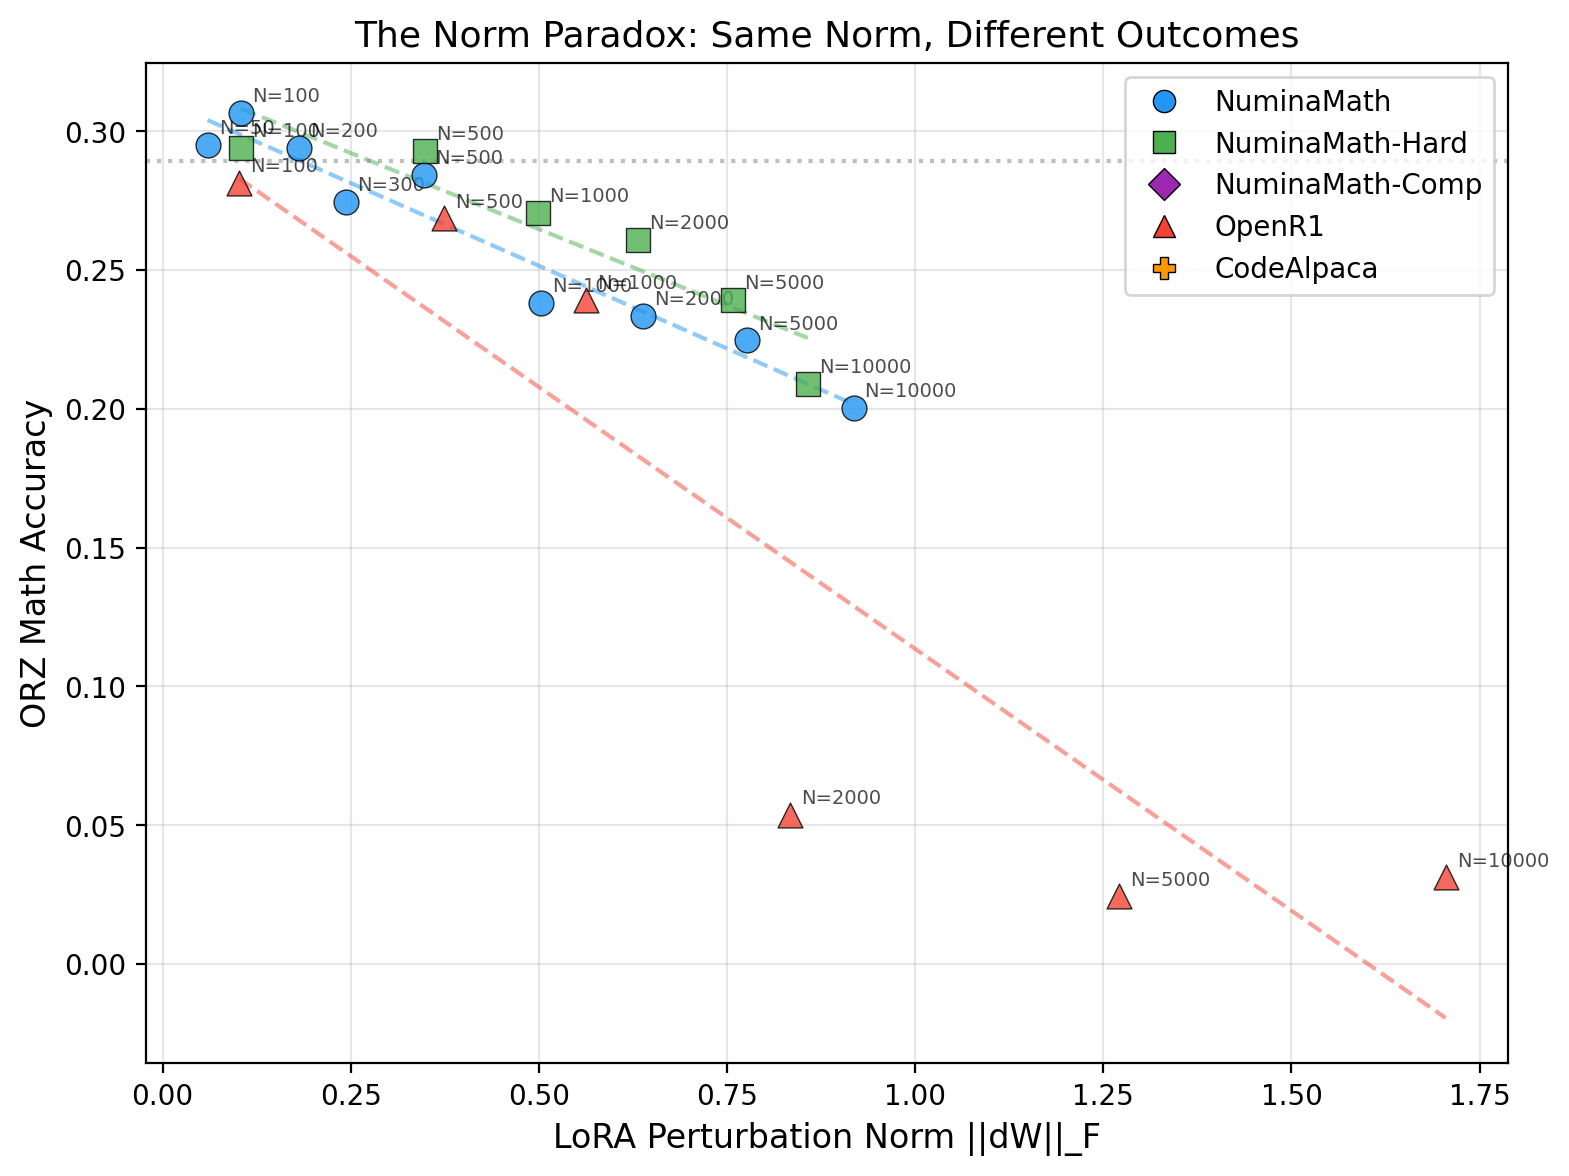
\includegraphics[width=\textwidth]{fig1_norm_vs_orz.png}
    \caption{$\|\Delta W\|_F$ vs ORZ accuracy. Within-source correlation is strong, but cross-source, the same norm produces vastly different outcomes.}
    \label{fig:norm-vs-orz}
\end{subfigure}
\hfill
\begin{subfigure}[t]{0.48\textwidth}
    \centering
    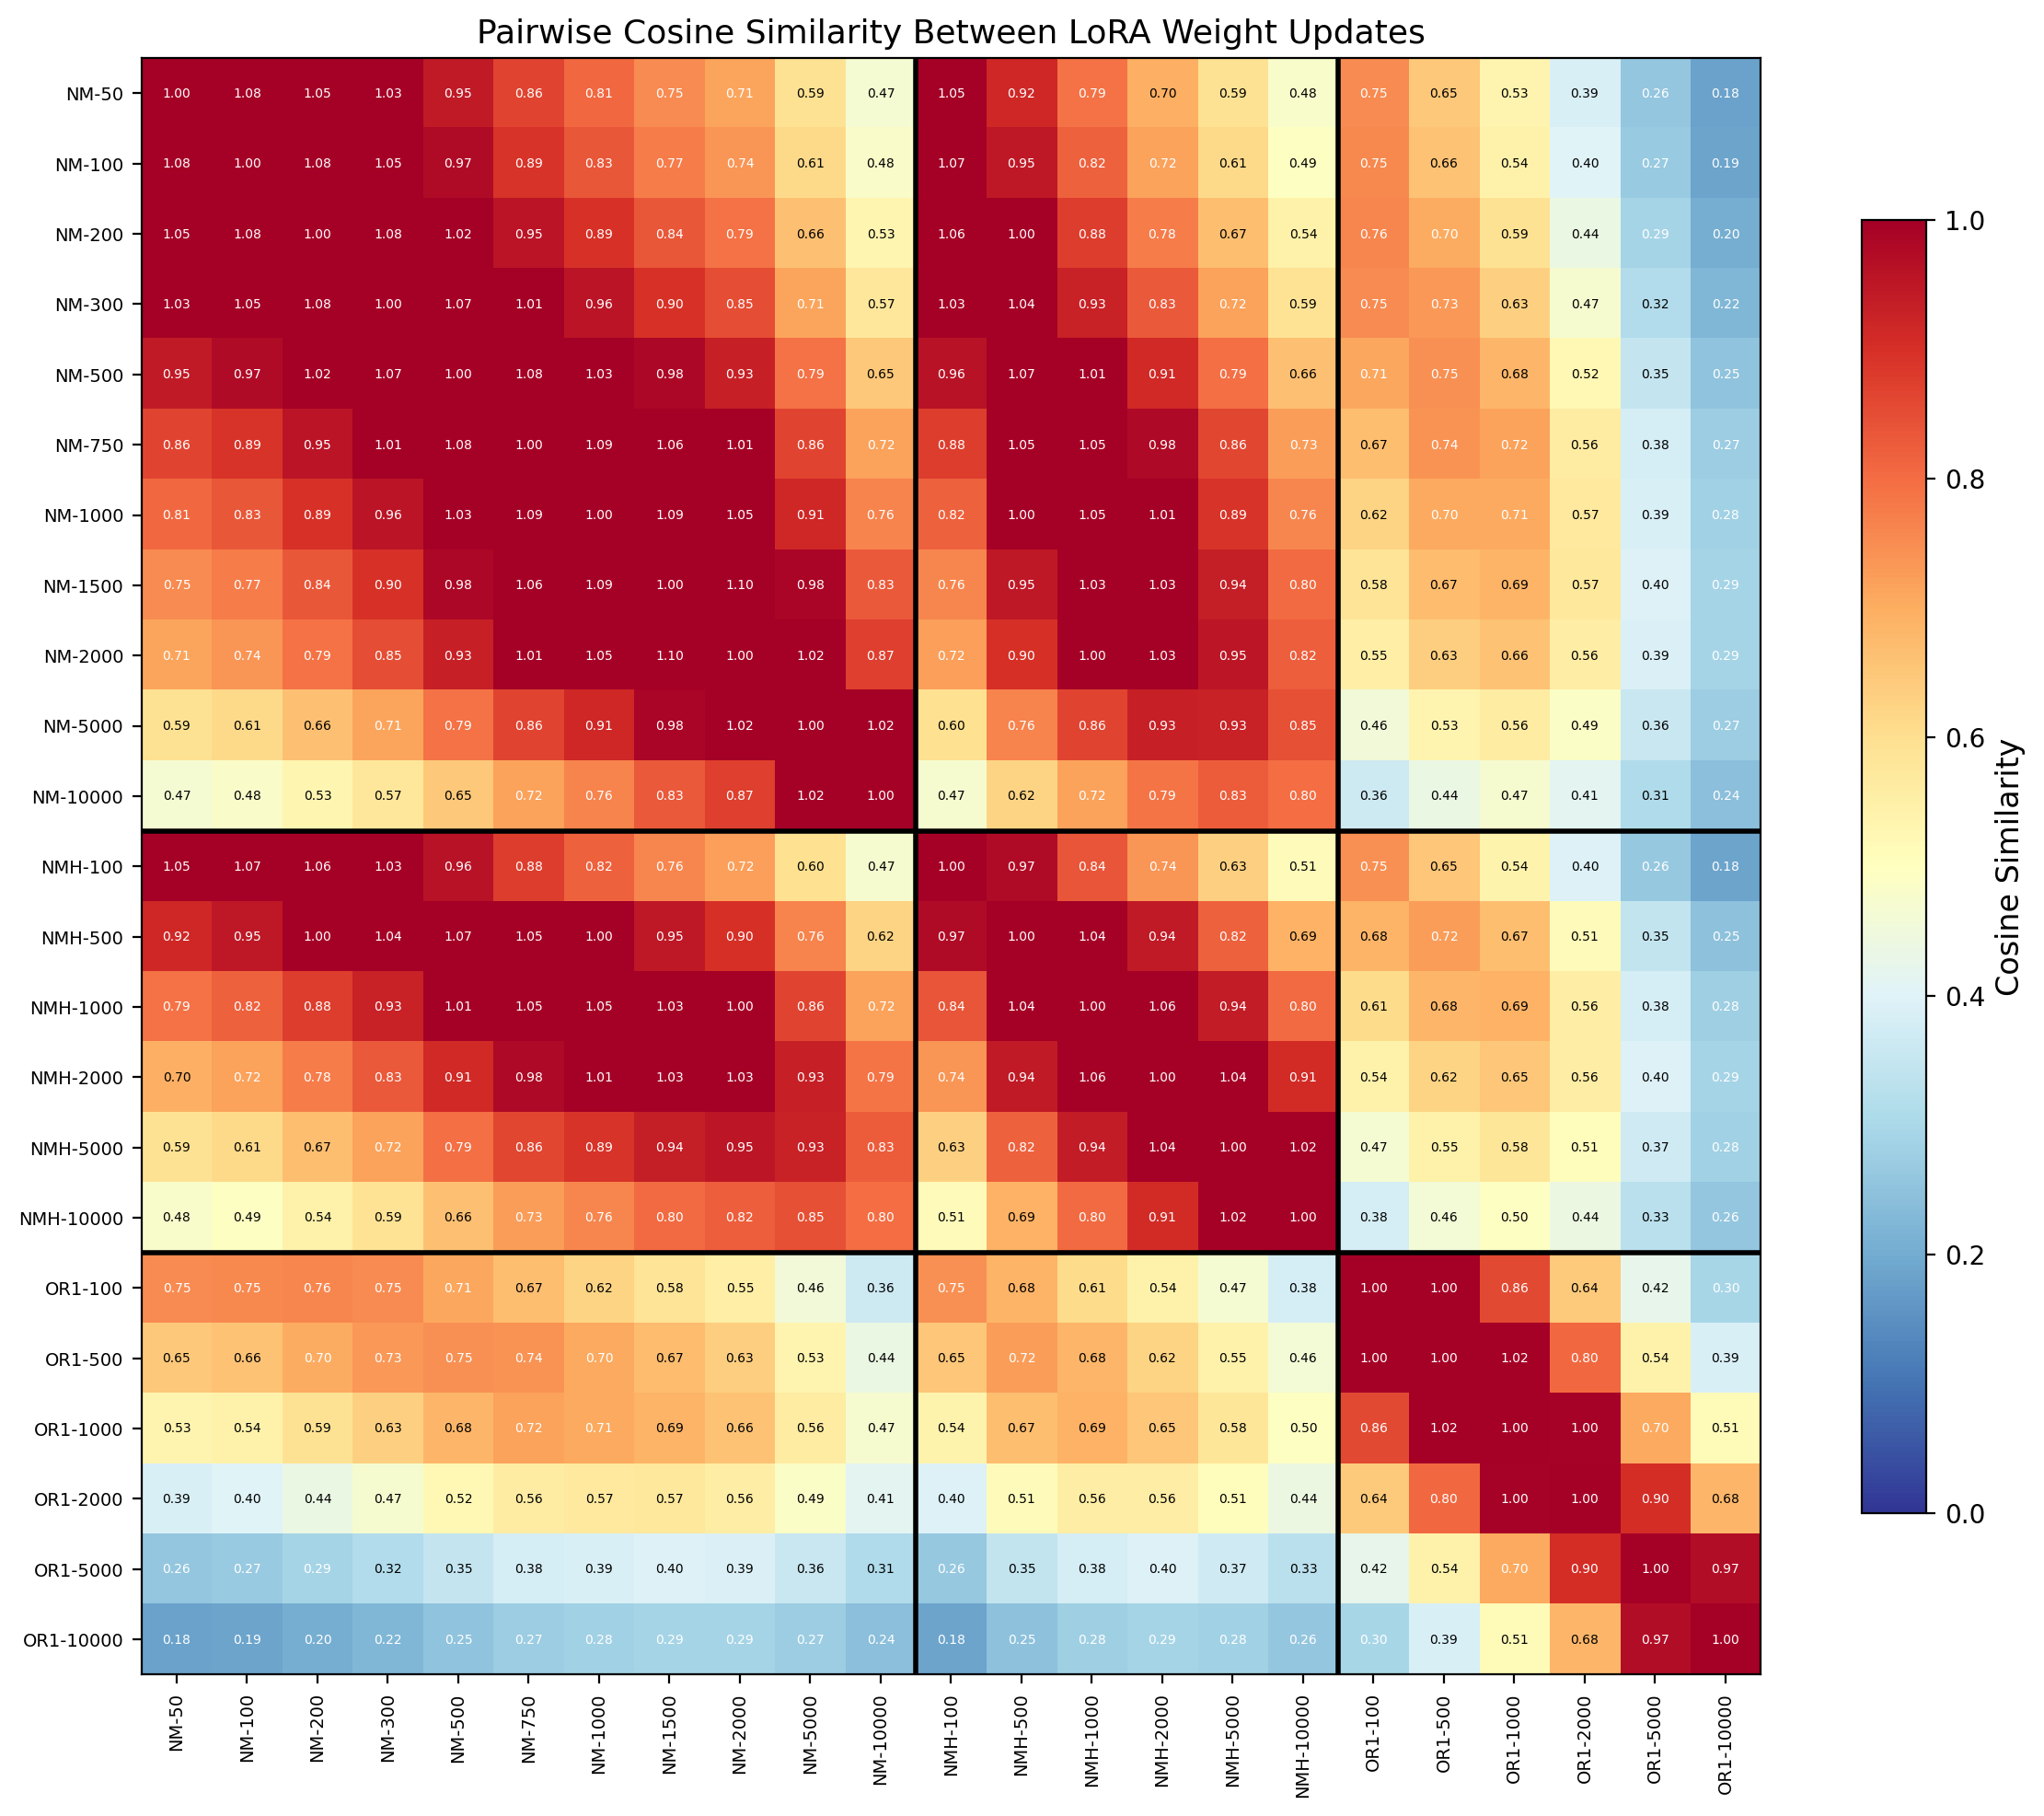
\includegraphics[width=\textwidth]{fig2_cosine_heatmap.png}
    \caption{Pairwise cosine similarity heatmap showing block structure by data source.}
    \label{fig:cosine-heatmap}
\end{subfigure}
\caption{The norm paradox and directional structure. (a)~Norm predicts accuracy within but not across sources. (b)~LoRA weight updates cluster by data source in weight space.}
\label{fig:main-results}
\end{figure}

%---------------------------------------------------------------------
\section{Degradation Mechanism: Format Disruption vs.\ Reasoning Loss}
\label{sec:mechanism}
%---------------------------------------------------------------------

Using strict vs.\ tolerant evaluation on GSM8K, we decompose total degradation into \textbf{format loss} (failing to produce \texttt{\textbackslash boxed\{\}} answers) and \textbf{reasoning loss} (incorrect reasoning regardless of format).

\subsection{NuminaMath: Gradual Reasoning Degradation}

NuminaMath exhibits a format phase transition between $N{=}500$ and $N{=}1{,}000$: boxed rate drops from 99.8\% to 82.0\%, causing 15.5\,pp of format-driven degradation. This recovers by $N{=}10{,}000$ (boxed rate 96.3\%), leaving only 6.9\,pp of cumulative reasoning loss.

\subsection{OpenR1: Catastrophic Format Collapse}

OpenR1 shows a qualitatively different pattern. The extended R1-style reasoning traces (16,469 chars avg) fundamentally alter the model's generation behavior.

\begin{table}[h]
\centering
\caption{OpenR1 GSM8K format decomposition. The transition between $N{=}1{,}500$ and $N{=}2{,}000$ is catastrophic.}
\label{tab:openr1-format}
\small
\begin{tabular}{@{}rrrrrr@{}}
\toprule
$N$ & Strict & Tolerant & Boxed Rate & Format Loss & Reasoning Loss \\
\midrule
100 & 84.2\% & 84.8\% & 100.0\% & $-0.8$\,pp & $+0.0$\,pp \\
500 & 83.4\% & 84.1\% & 99.8\% & $-0.7$\,pp & $+0.6$\,pp \\
1,000 & 77.2\% & 82.6\% & 94.5\% & $+5.5$\,pp & $+1.4$\,pp \\
1,500 & 83.0\% & 83.6\% & 99.6\% & $-0.6$\,pp & $+1.0$\,pp \\
\textbf{2,000} & \textbf{33.1\%} & \textbf{55.3\%} & \textbf{39.9\%} & \textbf{+22.2\,pp} & \textbf{+6.4\,pp} \\
5,000 & 33.7\% & 51.9\% & 37.2\% & $+18.3$\,pp & $+13.8$\,pp \\
10,000 & 50.0\% & 60.9\% & 56.4\% & $+10.8$\,pp & $+12.3$\,pp \\
\bottomrule
\end{tabular}
\end{table}

The cliff is remarkably sharp: $N{=}1{,}500$ shows completely normal behavior (strict GSM8K 83.0\%, boxed rate 99.6\%), yet just 500 additional training samples cause catastrophic collapse (strict 33.1\%, boxed rate 39.9\%). Format loss alone accounts for 22.2\,pp at $N{=}2{,}000$---the model can still compute correct answers (tolerant score 55.3\%) but fails to wrap them in \texttt{\textbackslash boxed\{\}}.

\subsection{Cross-Domain Robustness}

Throughout all 84 experiments, cross-domain tasks (SciKnowEval, ToolAlpaca) remain remarkably stable. Even OpenR1 at $N{=}10{,}000$ only degrades SciKnowEval by 7\,pp and ToolAlpaca negligibly. LoRA perturbations are confined to a task-relevant subspace.

%---------------------------------------------------------------------
\section{A Geometric Framework for SFT Degradation}
\label{sec:framework}
%---------------------------------------------------------------------

We propose that SFT degradation on capability $C$ follows:
\begin{equation}
\text{degradation}_C(\Delta W) = g\!\left(\left\|\text{proj}(\Delta W, V_C)\right\|\right)
\end{equation}
where $V_C$ is the subspace associated with capability $C$ and $g$ is monotonically increasing. The projection magnitude depends on both $\|\Delta W\|$ and the angle between $\Delta W$ and $V_C$:
\begin{equation}
\left\|\text{proj}(\Delta W, V_C)\right\| = \|\Delta W\| \cdot \left|\cos(\Delta W, V_C)\right|
\end{equation}

\textbf{Predictions:} (1)~Within-source linearity: if direction is constant, degradation $\approx f(\|\Delta W\|)$ alone, explaining $R^2 > 0.80$. (2)~Cross-source offsets: different directions produce different projections onto $V_C$. (3)~Cross-domain orthogonality: math SFT has near-zero projection onto chemistry/tool-use subspaces. (4)~$N$-dependent divergence: source choice matters more at higher $N$. All four are confirmed empirically.

\paragraph{Degradation efficiency.} We define $\eta = (\text{baseline} - \text{acc}) / \|\Delta W\|_F$. At $N{=}2{,}000$: NuminaMath $\eta = 0.093$, NuminaMath-Hard $\eta = 0.047$, OpenR1 $\eta = 0.298$, CodeAlpaca $\eta = 0.022$. OpenR1's efficiency is 13.5$\times$ higher than CodeAlpaca despite CodeAlpaca having 1.3$\times$ larger $\|\Delta W\|$---direction dominates.

%---------------------------------------------------------------------
\section{The OpenR1 Cliff: A Case Study in Directional Catastrophe}
\label{sec:cliff}
%---------------------------------------------------------------------

\subsection{Characterizing the Transition}

Fine-grained experiments precisely localize the transition (Figure~\ref{fig:cliff}):

\begin{table}[h]
\centering
\caption{The OpenR1 cliff. Three things happen simultaneously between $N{=}1{,}500$ and $N{=}2{,}000$.}
\label{tab:cliff}
\small
\begin{tabular}{@{}rrrrrr@{}}
\toprule
$N$ & ORZ & GSM8K (strict) & Boxed Rate & $\|\Delta W\|$ & $\cos(\text{NM})$ \\
\midrule
1,000 & 23.9\% & 77.2\% & 94.5\% & 0.53 & 0.71 \\
1,250 & 25.7\% & 83.5\% & 99.7\% & 0.44 & -- \\
1,500 & 25.9\% & 83.0\% & 99.6\% & 0.49 & -- \\
\textbf{2,000} & \textbf{5.4\%} & \textbf{33.1\%} & \textbf{39.9\%} & \textbf{0.79} & \textbf{0.56} \\
5,000 & 2.4\% & 33.7\% & 37.2\% & 1.21 & 0.36 \\
\bottomrule
\end{tabular}
\end{table}

\subsection{Seed Replication}

To confirm this is not a seed artifact, we replicate with 4 random seeds. All show catastrophic collapse: ORZ $= 4.50\% \pm 0.87$ (range 3.5--5.4\%). The standard deviation is small relative to the 24\,pp mean drop from baseline.

\begin{figure}[t]
\centering
\begin{subfigure}[t]{0.48\textwidth}
    \centering
    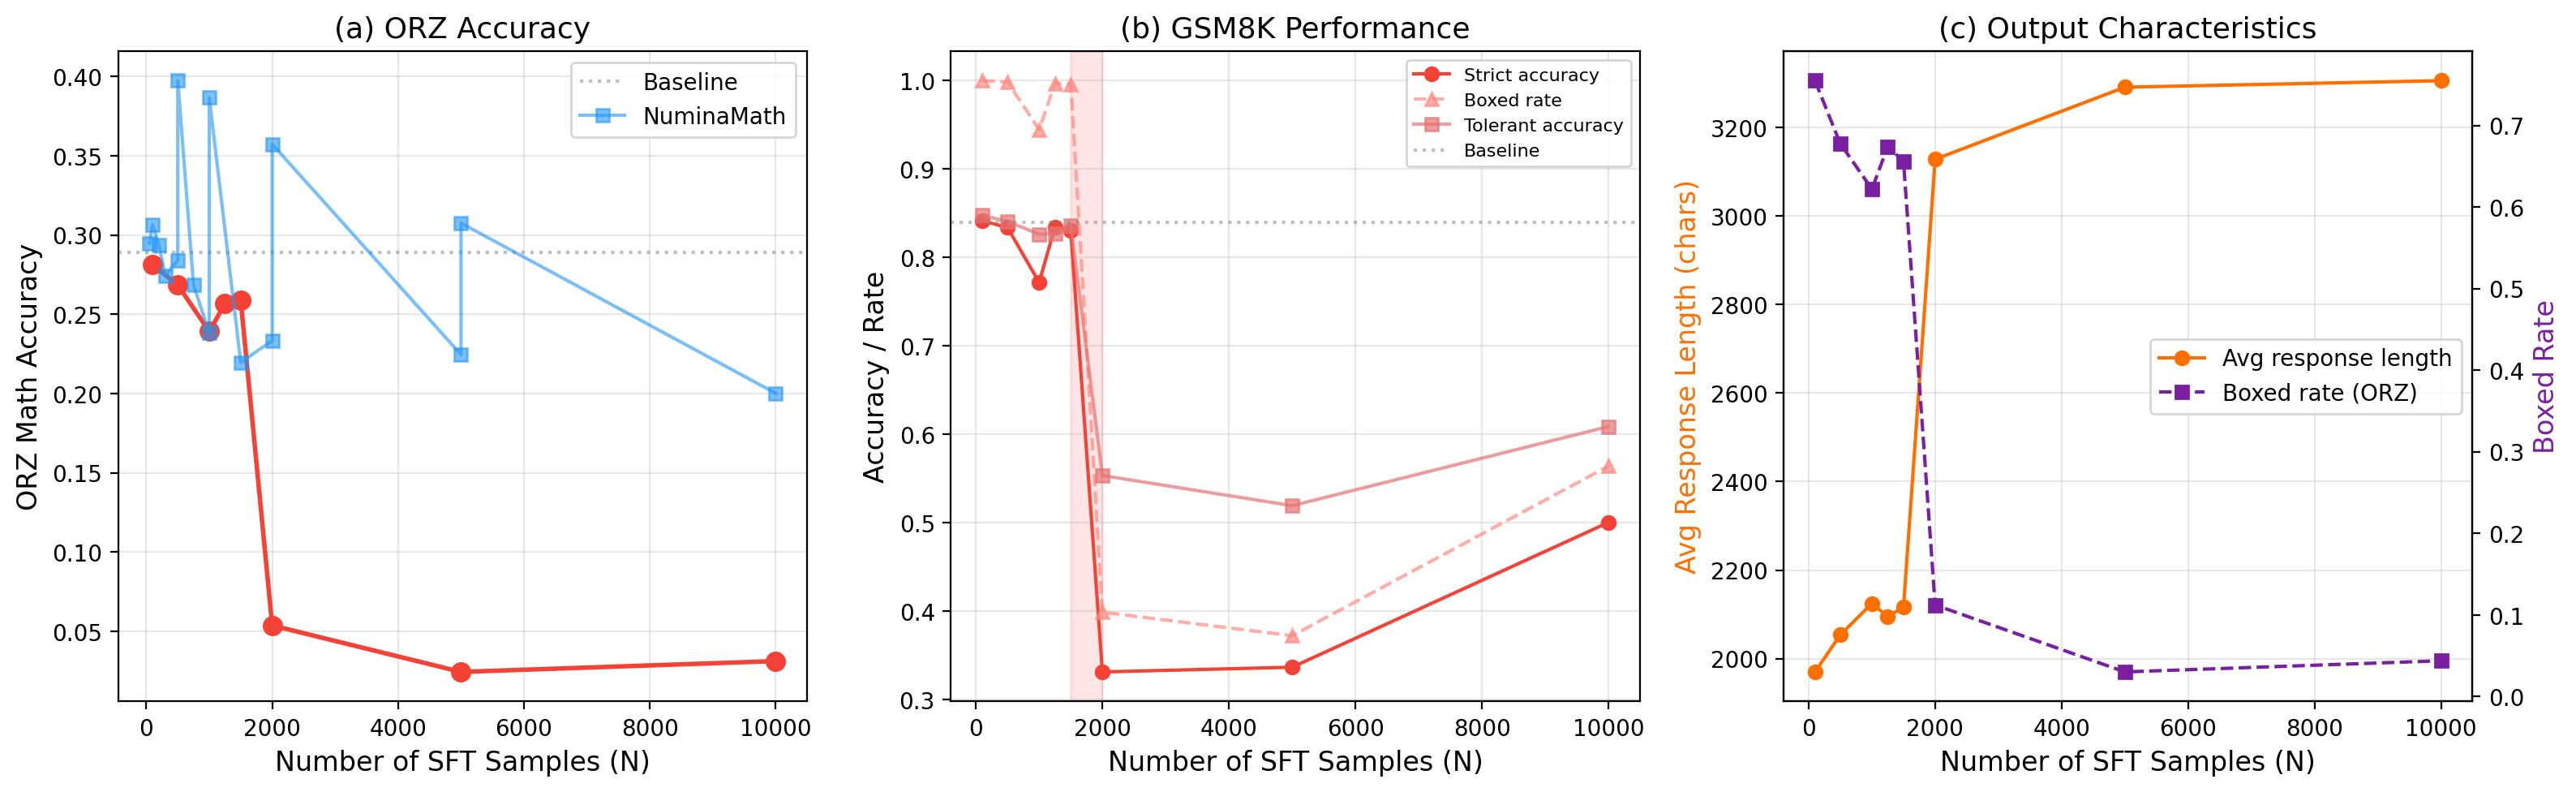
\includegraphics[width=\textwidth]{fig6_openr1_cliff.png}
    \caption{The OpenR1 cliff: ORZ, GSM8K boxed rate, and response length vs $N$.}
    \label{fig:cliff}
\end{subfigure}
\hfill
\begin{subfigure}[t]{0.48\textwidth}
    \centering
    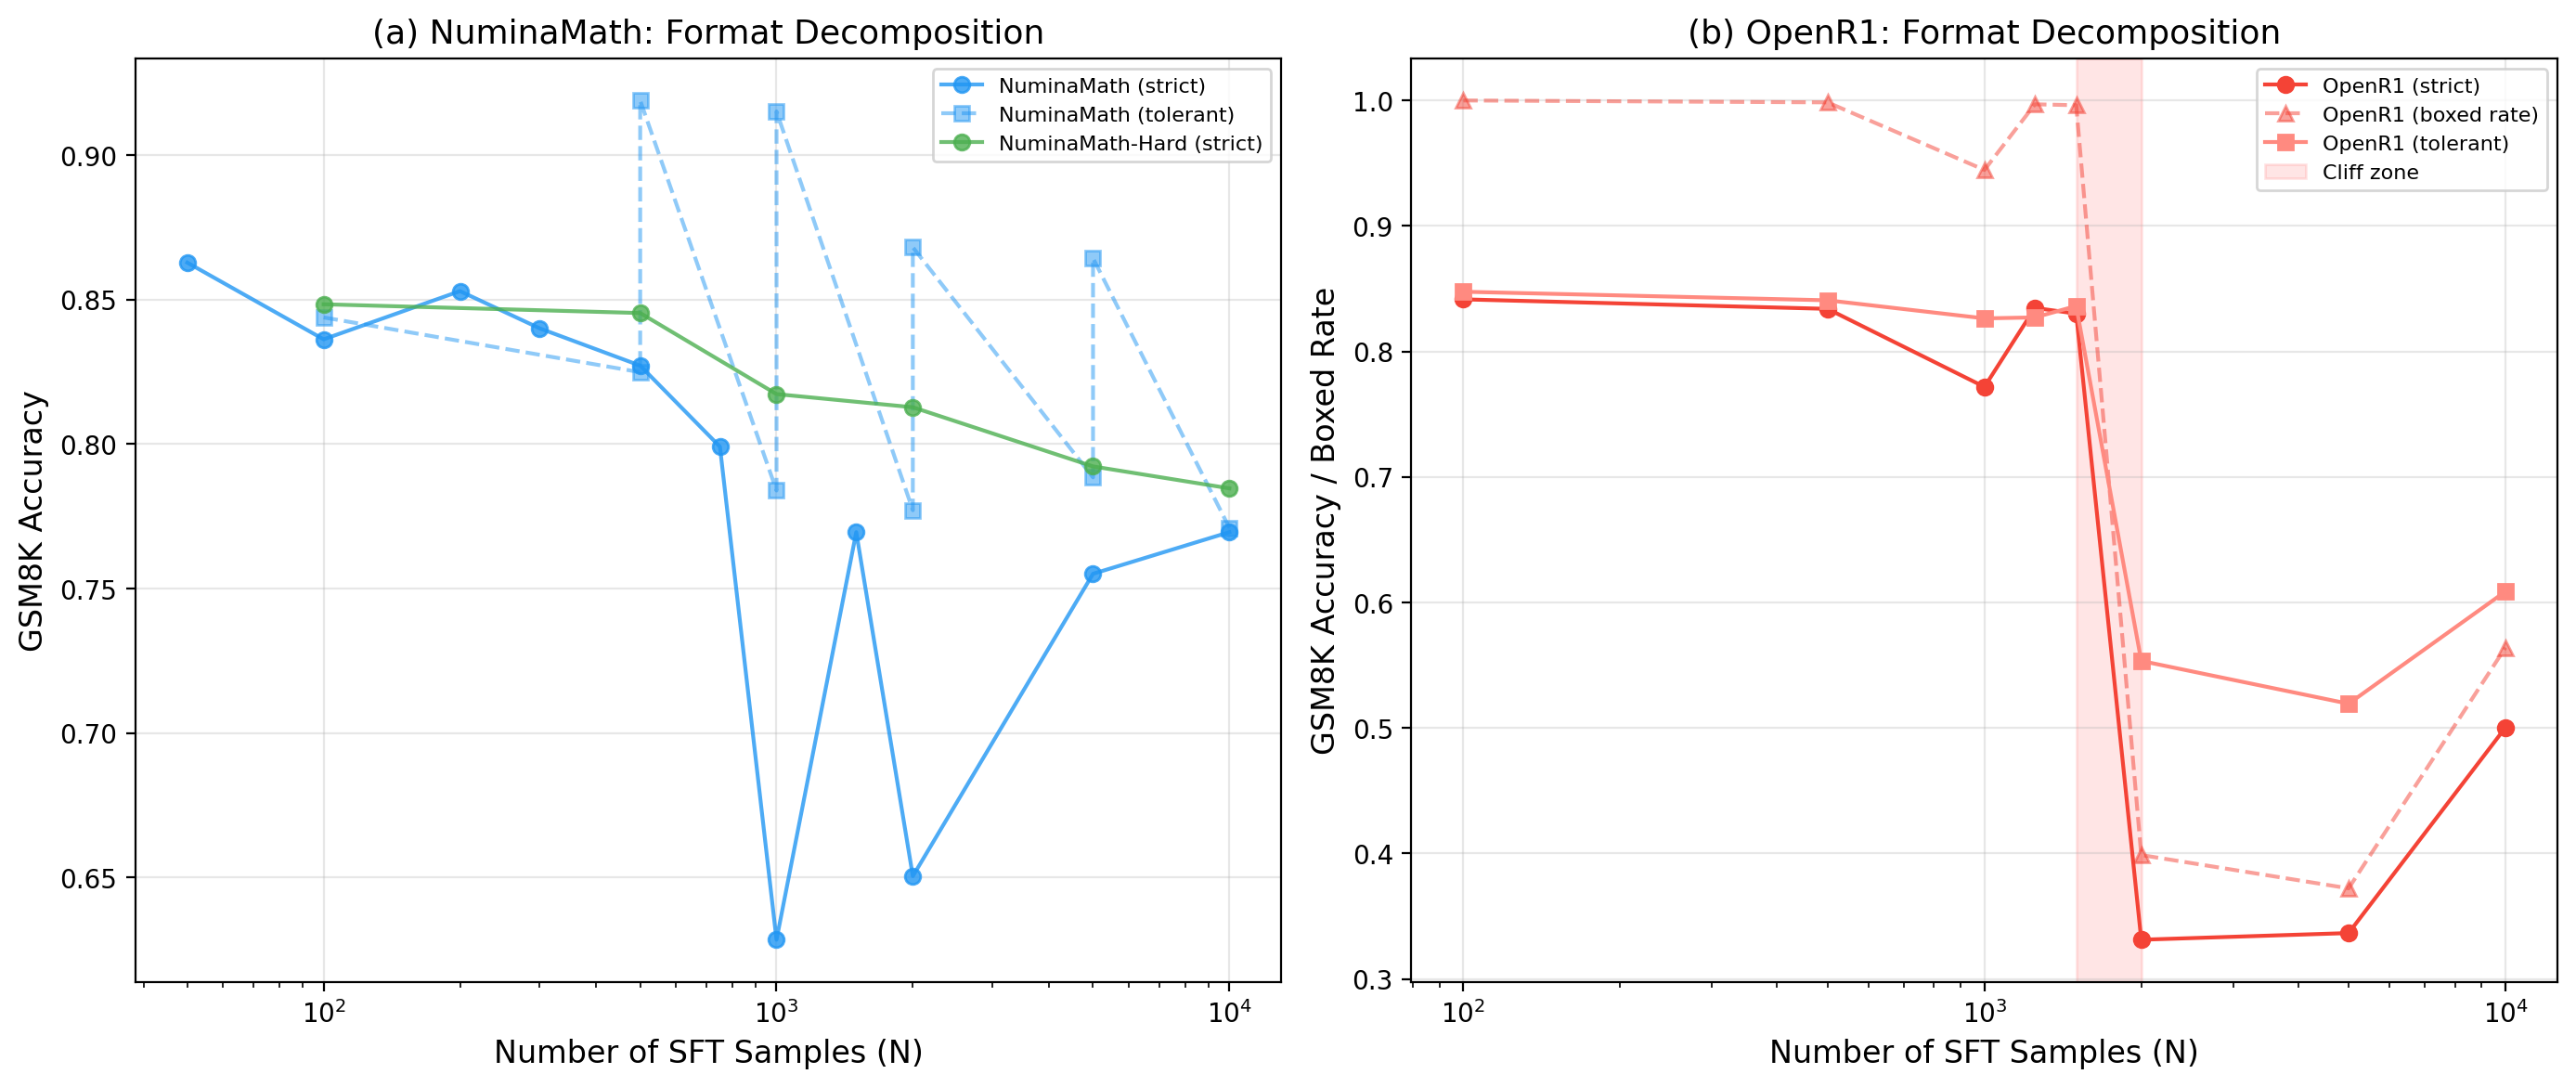
\includegraphics[width=\textwidth]{fig5_format_decomposition.png}
    \caption{Format vs reasoning decomposition for NuminaMath and OpenR1.}
    \label{fig:format-decomp}
\end{subfigure}
\caption{The OpenR1 cliff and format decomposition. (a)~Catastrophic collapse between $N{=}1{,}500$ and $N{=}2{,}000$. (b)~Format loss dominates at the cliff; reasoning loss is cumulative.}
\end{figure}

\subsection{Truncation Control}

To disentangle content from style, we truncate OpenR1 solutions to NuminaMath-like length (${\sim}1{,}500$ chars) while preserving the \texttt{\textbackslash boxed\{\}} answer.

\begin{table}[h]
\centering
\caption{Truncation control. Truncation mitigates the cliff but doesn't eliminate the gap.}
\label{tab:truncation}
\small
\begin{tabular}{@{}rrrr@{}}
\toprule
$N$ & Trunc-OR1 & Full OR1 & NuminaMath \\
\midrule
1,000 & 25.6\% & 23.9\% & 23.8\% \\
2,000 & \textbf{11.7\%} & 5.4\% & 23.3\% \\
5,000 & 15.2\% & 2.4\% & 22.5\% \\
\bottomrule
\end{tabular}
\end{table}

Truncation substantially mitigates the collapse (11.7\% vs 5.4\% at $N{=}2{,}000$), but truncated OpenR1 still degrades more than NuminaMath (11.7\% vs 23.3\%). This shows \textbf{direction has both a content component and a style component}: style/length accounts for roughly half the gap.

\subsection{Data Mixing}

We test whether perturbation direction can be steered by mixing NuminaMath and OpenR1 at $N{=}2{,}000$ total.

\begin{table}[h]
\centering
\caption{Data mixing at $N{=}2{,}000$. Both accuracy and direction interpolate smoothly.}
\label{tab:mixing}
\small
\begin{tabular}{@{}lrrrr@{}}
\toprule
Mix (NM/OR1) & ORZ & Boxed Rate & $\|\Delta W\|$ & $\cos(\Delta W, \text{NM-ref})$ \\
\midrule
100/0 (pure NM) & 23.3\% & 82.3\% & 0.60 & 0.87 \\
75/25 & 23.2\% & 82.3\% & 0.65 & 0.72 \\
50/50 & 21.3\% & 82.9\% & 0.71 & 0.59 \\
25/75 & 19.9\% & 70.8\% & 0.75 & 0.49 \\
0/100 (pure OR1) & 5.4\% & 39.9\% & 0.79 & 0.41 \\
\bottomrule
\end{tabular}
\end{table}

ORZ accuracy interpolates smoothly (23.3\% $\to$ 5.4\%) while the cosine with the NM reference direction decreases monotonically (0.87 $\to$ 0.41). Format compliance shows a threshold at ${\sim}75\%$ OpenR1 fraction. This confirms direction is a continuous, manipulable quantity.

%---------------------------------------------------------------------
\section{Multi-Scale Analysis: Qwen2.5-7B}
\label{sec:7b}
%---------------------------------------------------------------------

We replicate core experiments at 7B scale (Figure~\ref{fig:7b}).

\begin{table}[h]
\centering
\caption{7B results. The OpenR1 cliff persists but shifts to higher $N$.}
\label{tab:7b}
\small
\begin{tabular}{@{}lrrrr@{}}
\toprule
& \multicolumn{2}{c}{NuminaMath} & \multicolumn{2}{c}{OpenR1} \\
\cmidrule(lr){2-3} \cmidrule(lr){4-5}
$N$ & ORZ & GSM8K-S & ORZ & GSM8K-S \\
\midrule
500 & 39.8\% & 91.8\% & 36.6\% & 91.3\% \\
1,000 & 38.7\% & 91.1\% & 35.2\% & 92.0\% \\
2,000 & 35.7\% & 71.3\% & 30.7\% & 90.9\% \\
5,000 & 30.8\% & 82.5\% & \textbf{4.6\%} & \textbf{56.5\%} \\
\bottomrule
\end{tabular}
\end{table}

Three key findings: (1)~NuminaMath shows smooth degradation at both scales. (2)~The OpenR1 cliff exists at 7B but shifts from $N{\sim}1{,}500$--$2{,}000$ (3B) to $N{\sim}2{,}000$--$5{,}000$ (7B)---the larger model absorbs more before collapse. (3)~Cross-domain benchmarks remain robust until the cliff.

%---------------------------------------------------------------------
\section{Cross-Domain Directional Analysis}
\label{sec:cross-domain}
%---------------------------------------------------------------------

To test whether the framework extends beyond math variants, we fine-tune on CodeAlpaca-20k.

\begin{figure}[t]
\centering
\begin{subfigure}[t]{0.48\textwidth}
    \centering
    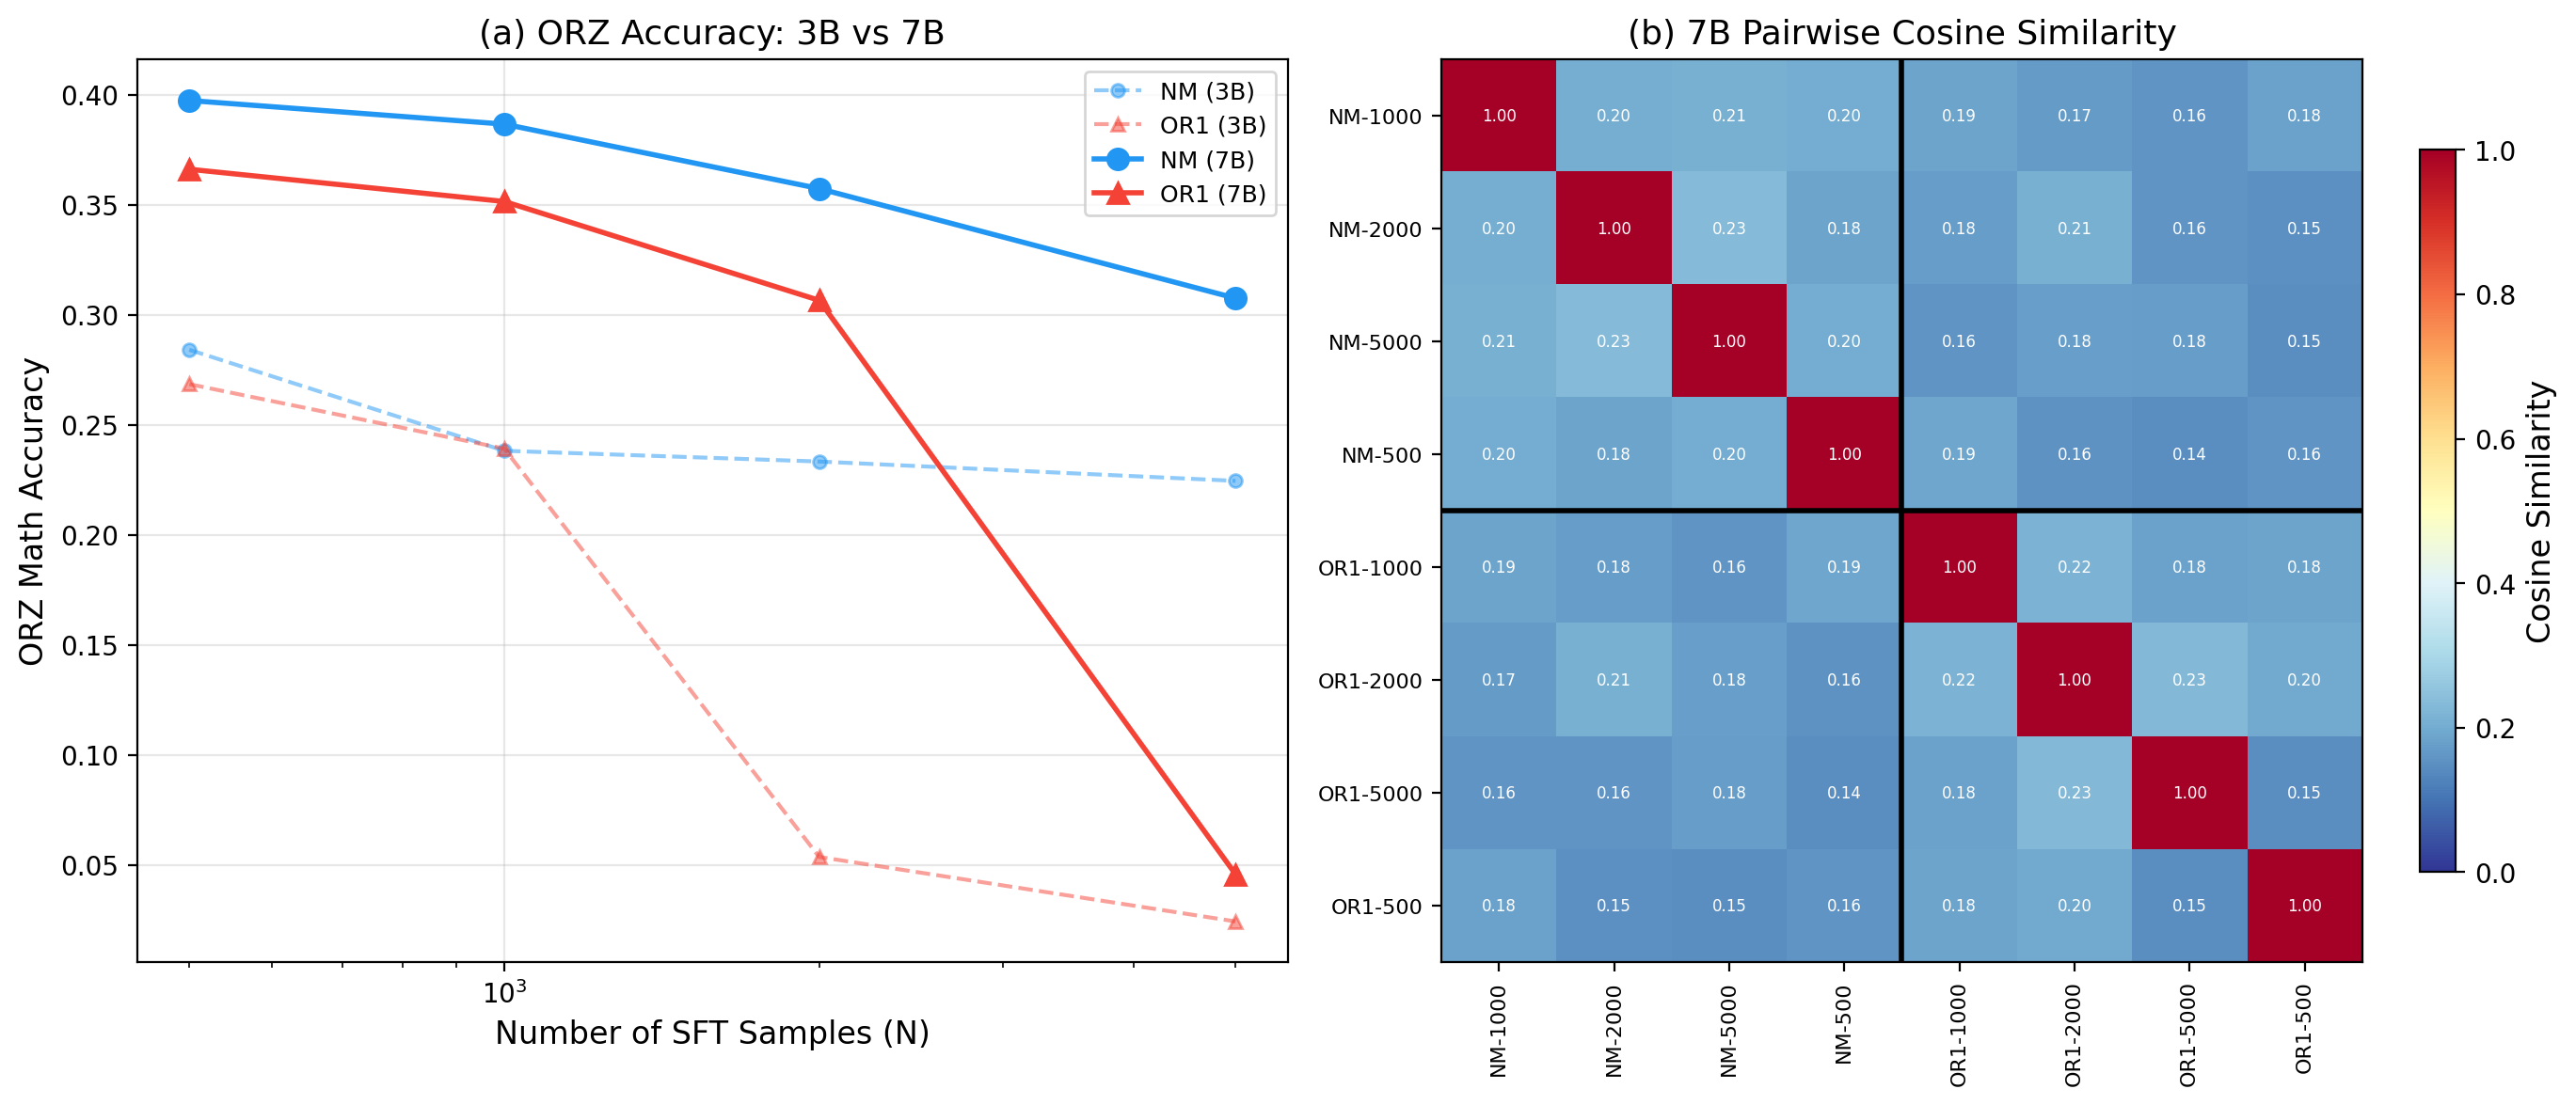
\includegraphics[width=\textwidth]{fig11_7b_comparison.png}
    \caption{7B scale replication. The OpenR1 cliff shifts to $N{=}5{,}000$.}
    \label{fig:7b}
\end{subfigure}
\hfill
\begin{subfigure}[t]{0.48\textwidth}
    \centering
    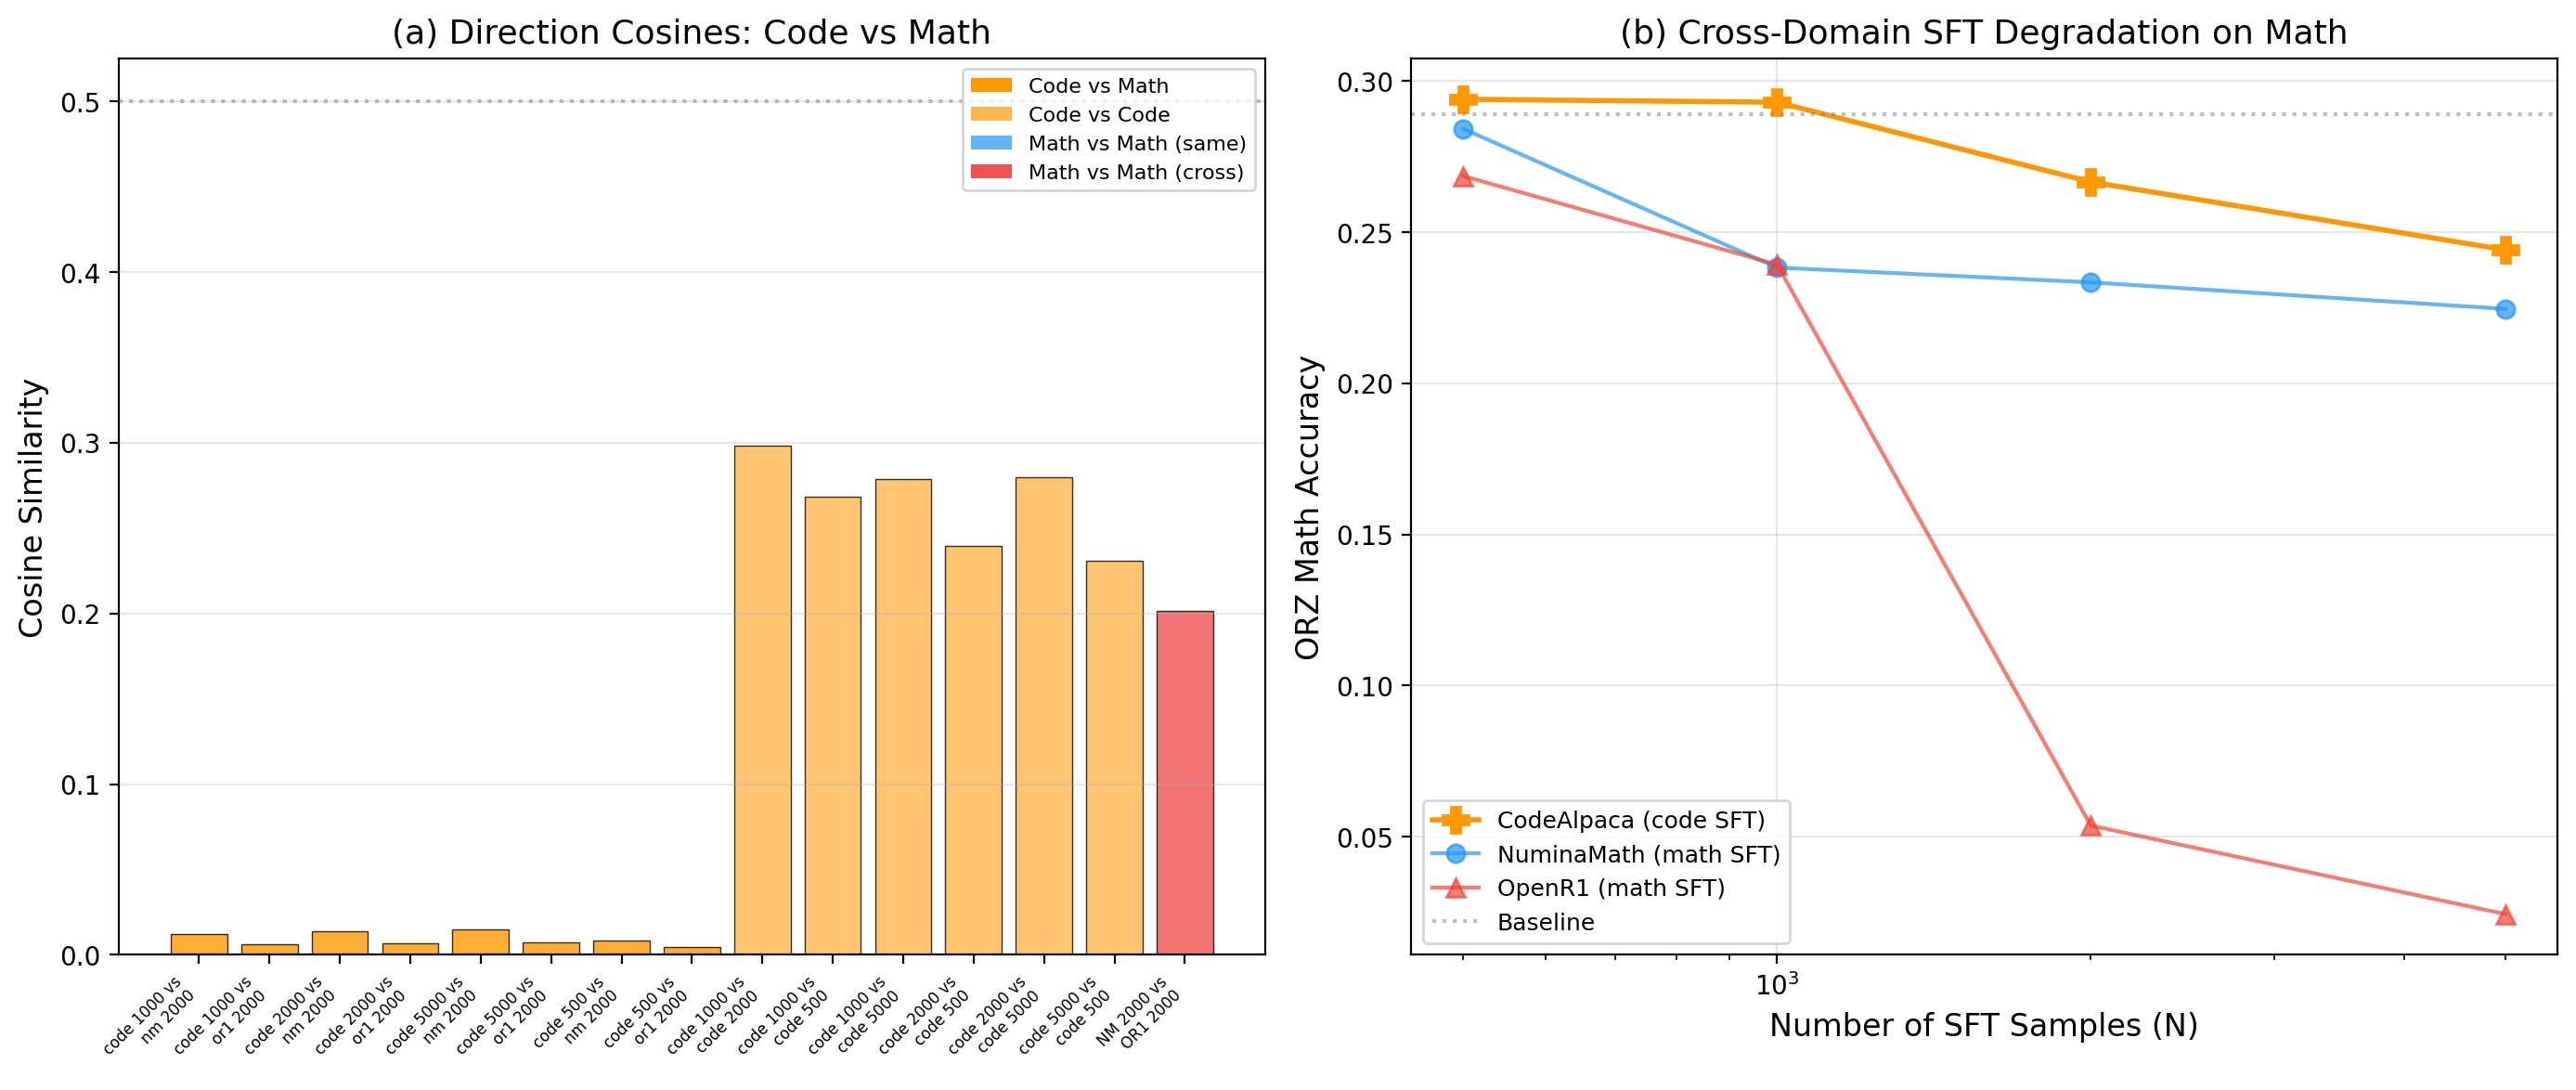
\includegraphics[width=\textwidth]{fig12_code_domain.png}
    \caption{CodeAlpaca directions are orthogonal to all math directions ($\cos{\sim}0.01$).}
    \label{fig:code}
\end{subfigure}
\caption{Generality of directional structure. (a)~Qualitative patterns preserved at 7B. (b)~Cross-domain SFT confirms near-orthogonal perturbation directions.}
\end{figure}

Code SFT directions are essentially orthogonal to all math directions (cos ${\sim} 0.01$). CodeAlpaca has the \emph{largest} perturbation norm ($\|\Delta W\| = 1.023$ at $N{=}2{,}000$, 1.7$\times$ NuminaMath) yet the \emph{smallest} math degradation ($-2.2$\,pp). Its degradation efficiency $\eta = 0.022$ is $13.5{\times}$ lower than OpenR1's---decisively confirming that direction, not magnitude, determines degradation.

%---------------------------------------------------------------------
\section{Statistical Robustness}
\label{sec:robustness}
%---------------------------------------------------------------------

\paragraph{NuminaMath seed variations.} We run 4 seeds at $N \in \{100, 500, 2{,}000, 10{,}000\}$. Seed variance is uniformly small (0.2--1.0\,pp) across all sample counts, while the degradation signal grows with $N$ (6+\,pp at $N{=}2{,}000$, 9+\,pp at $N{=}10{,}000$).

\paragraph{OpenR1 cliff seeds.} All 4 seeds at $N{=}2{,}000$ show catastrophic collapse: ORZ $= 4.50\% \pm 0.87$ (range 3.5--5.4\%), GSM8K strict $= 37.3\% \pm 3.8$, confirming this is a systematic phenomenon.

\paragraph{Hyperparameter sensitivity.} Aggressive hyperparameters ($r{=}16$, LR$=2{\times}10^{-4}$, 3 epochs) amplify perturbation magnitude but preserve direction. The direction is a property of the data source, not the optimizer.

%---------------------------------------------------------------------
\section{Practical Implications}
%---------------------------------------------------------------------

\textbf{Pre-SFT direction probes.} Train a cheap LoRA probe (small $N$) and compare its weight-update direction to known-good directions. High cosine similarity predicts safe degradation profiles.

\textbf{Data source selection.} The degradation efficiency metric $\eta$ provides actionable guidance: NuminaMath-Hard ($\eta = 0.047$) is 6.3$\times$ safer per unit norm than OpenR1 ($\eta = 0.298$).

\textbf{Format monitoring.} Separately track format compliance and reasoning accuracy. Format disruption is recoverable by training longer; reasoning degradation is not.

%---------------------------------------------------------------------
\section{Limitations}
%---------------------------------------------------------------------

\textbf{Two model scales.} We test on 3B and 7B from the Qwen2.5 family. Generalization to other architectures and much larger scales remains untested.

\textbf{Capability subspace not directly observed.} We infer $V_C$ indirectly from degradation patterns. A direct characterization via activation patching or causal tracing would provide stronger evidence.

\textbf{Limited domain diversity.} We include CodeAlpaca but have not tested other domains (dialogue, summarization, multilingual).

%---------------------------------------------------------------------
\section{Conclusion}
%---------------------------------------------------------------------

We have shown that SFT-induced degradation is fundamentally a \emph{directional} phenomenon in weight space. Within a data source, perturbation magnitude predicts degradation with $R^2 > 0.80$. Across sources, the same magnitude produces vastly different outcomes (4$\times$ degradation gap at matched norms), explained by source-dependent perturbation directions that diverge as training volume increases.

The geometric framework---degradation depends on the projection of the weight update onto capability-specific subspaces---unifies within-source norm scaling, cross-source degradation gaps, cross-domain robustness, format phase transitions, and the OpenR1 catastrophic cliff.

Our cross-domain experiments provide the strongest evidence: CodeAlpaca code SFT produces near-orthogonal perturbation directions ($\cos{\sim}0.01$) with the largest weight update norms, yet the smallest math degradation. \textbf{Direction, not magnitude, determines which capabilities are affected.} The OpenR1 cliff reproduces across 4 seeds ($4.50\% \pm 0.87$) and at 7B scale (shifted to $N{\sim}5{,}000$), confirming it as a systematic phenomenon.

For practitioners: \textbf{not all perturbations are equal.} Choosing training data that produces perturbations aligned with the target task but orthogonal to capabilities you want to preserve is the geometric principle underlying successful SFT.

%---------------------------------------------------------------------
% References
%---------------------------------------------------------------------
\bibliographystyle{plainnat}

\begin{thebibliography}{11}

\bibitem[Biderman et~al.(2024)]{biderman2024lora}
D.~Biderman, J.~Portes, J.~G.~Ortiz, M.~Greber, G.~L.~Doney, S.~Shahsavari, H.~Patel, K.~Scheible, C.~Kacmarcik, and L.~Hestness.
\newblock {LoRA} learns less and forgets less.
\newblock \emph{arXiv:2405.09673}, 2024.

\bibitem[Chen et~al.(2023)]{chen2023alpagasus}
L.~Chen, S.~Li, J.~Yan, H.~Wang, K.~Gunaratna, V.~Yadav, Z.~Tang, V.~Srinivasan, T.~Zhou, H.~Huang, and H.~Jin.
\newblock {AlpaGasus}: Training a better {Alpaca} with fewer data.
\newblock \emph{arXiv:2307.08701}, 2023.

\bibitem[Chaudhary(2023)]{chaudhary2023codealpaca}
S.~Chaudhary.
\newblock {CodeAlpaca}: An instruction-following {LLaMA} model for code generation, 2023.

\bibitem[Hu et~al.(2022)]{hu2022lora}
E.~J.~Hu, Y.~Shen, P.~Wallis, Z.~Allen-Zhu, Y.~Li, S.~Wang, L.~Wang, and W.~Chen.
\newblock {LoRA}: Low-rank adaptation of large language models.
\newblock In \emph{ICLR}, 2022.

\bibitem[Kirkpatrick et~al.(2017)]{kirkpatrick2017overcoming}
J.~Kirkpatrick, R.~Pascanu, N.~Rabinowitz, J.~Veres, G.~Desjardins, A.~A.~Rusu, K.~Milan, J.~Quan, T.~Ramalho, A.~Grabska-Barwinska, et~al.
\newblock Overcoming catastrophic forgetting in neural networks.
\newblock \emph{PNAS}, 114(13), 2017.

\bibitem[Li et~al.(2018)]{li2018measuring}
H.~Li, Z.~Xu, G.~Taylor, C.~Studer, and T.~Goldstein.
\newblock Measuring the intrinsic dimension of objective landscapes.
\newblock In \emph{ICLR}, 2018.

\bibitem[Li et~al.(2024)]{li2024numinamath}
Y.~Li et~al.
\newblock {NuminaMath}: A large-scale curated dataset for mathematical reasoning, 2024.

\bibitem[Luo et~al.(2023)]{luo2023empirical}
Y.~Luo, Z.~Yang, F.~Meng, Y.~Li, J.~Zhou, and Y.~Zhang.
\newblock An empirical study of catastrophic forgetting in large language models during continual fine-tuning.
\newblock \emph{arXiv:2308.08747}, 2023.

\bibitem[{Open-Reasoner}(2024)]{openr1}
{Open-Reasoner}.
\newblock {OpenR1-Math}: High-quality math reasoning data from {R1} distillation, 2024.

\bibitem[Yang et~al.(2024)]{yang2024qwen}
A.~Yang et~al.
\newblock {Qwen2.5} technical report.
\newblock \emph{arXiv:2412.15115}, 2024.

\bibitem[Zhou et~al.(2023)]{zhou2023lima}
C.~Zhou, P.~Liu, P.~Xu, S.~Iyer, J.~Sun, Y.~Mao, X.~Ma, A.~Efrat, P.~Yu, L.~Yu, S.~Zhang, G.~Ghosh, M.~Lewis, L.~Zettlemoyer, and O.~Levy.
\newblock {LIMA}: Less is more for alignment.
\newblock In \emph{NeurIPS}, 2023.

\end{thebibliography}

%---------------------------------------------------------------------
\newpage
\appendix
\section{Complete Experimental Results}
\label{app:results}

\subsection{NuminaMath Standard Config ($r{=}8$, LR$=5{\times}10^{-5}$, 1 epoch)}

\begin{table}[h]
\centering
\small
\begin{tabular}{@{}rrrrrr@{}}
\toprule
$N$ & ORZ & $\|\Delta W\|_F$ & SciKnow & TA-Real F & Valid \\
\midrule
50 & 29.5\% & 0.056 & 34.0\% & 89\% & Y \\
100 & 30.7\% & 0.098 & 35.2\% & 89\% & Y \\
200 & 29.4\% & 0.172 & 33.4\% & 89\% & Y \\
300 & 27.4\% & 0.230 & 33.8\% & 89\% & Y \\
500 & 28.4\% & 0.330 & 35.3\% & 89\% & Y \\
750 & 26.9\% & 0.410 & 31.9\% & 89\% & Y \\
1,000 & 23.8\% & 0.478 & 32.6\% & 88\% & Y \\
1,500 & 22.0\% & 0.551 & 32.0\% & 89\% & Y \\
2,000 & 23.3\% & 0.604 & 31.6\% & 89\% & Y \\
5,000 & 22.5\% & 0.733 & 33.8\% & 91\% & Y \\
10,000 & 20.0\% & 0.869 & 31.5\% & 90\% & Y \\
\bottomrule
\end{tabular}
\end{table}

\subsection{OpenR1 Standard Config}

\begin{table}[h]
\centering
\small
\begin{tabular}{@{}rrrrrr@{}}
\toprule
$N$ & ORZ & $\|\Delta W\|_F$ & SciKnow & TA-Real F & Valid \\
\midrule
100 & 28.1\% & 0.096 & 34.6\% & 89\% & Y \\
500 & 26.9\% & 0.356 & 34.9\% & 88\% & Y \\
1,000 & 23.9\% & 0.529 & 33.7\% & 86\% & N \\
1,250 & 25.7\% & 0.445 & 33.4\% & 89\% & Y \\
1,500 & 25.9\% & 0.489 & 32.0\% & 87\% & Y \\
2,000 & 5.4\% & 0.789 & 35.8\% & 86\% & N \\
5,000 & 2.4\% & 1.211 & 30.1\% & 89\% & N \\
10,000 & 3.1\% & 1.628 & 27.4\% & 89\% & N \\
\bottomrule
\end{tabular}
\end{table}

\subsection{Seed Variation Details}

\begin{table}[h]
\centering
\small
\caption{NuminaMath seed variations (standard config).}
\begin{tabular}{@{}rrrr@{}}
\toprule
$N$ & Seeds & ORZ Mean $\pm$ Std & Range \\
\midrule
100 & 4 & 29.6\% $\pm$ 1.0 & 28.5--30.7\% \\
500 & 4 & 28.4\% $\pm$ 0.2 & 28.0--28.6\% \\
2,000 & 4 & 22.6\% $\pm$ 0.5 & 22.2--23.3\% \\
10,000 & 4 & 19.9\% $\pm$ 0.5 & 19.0--20.5\% \\
\bottomrule
\end{tabular}
\end{table}

\begin{table}[h]
\centering
\small
\caption{OpenR1 $N{=}2{,}000$ cliff replication across 4 seeds.}
\begin{tabular}{@{}rrrr@{}}
\toprule
Seed & ORZ & GSM8K Strict & SciKnow \\
\midrule
42 & 5.37\% & 33.1\% & 35.8\% \\
1 & 3.52\% & 40.9\% & 32.8\% \\
2 & 3.91\% & 40.2\% & 31.3\% \\
3 & 5.18\% & 34.9\% & 33.3\% \\
\midrule
Mean $\pm$ Std & 4.50 $\pm$ 0.87 & 37.3 $\pm$ 3.8 & 33.3 $\pm$ 1.8 \\
\bottomrule
\end{tabular}
\end{table}

\end{document}
